\documentclass[10pt,a4paper, final]{article}
\usepackage[utf8]{inputenc}

\usepackage[a4paper]{geometry}

\usepackage{amsmath}
\usepackage{amsfonts}
\usepackage{amssymb}
\usepackage{booktabs}

\usepackage{graphicx}

\usepackage{standalone}
\usepackage{datetime}

\usepackage[defernumbers=true]{biblatex}
\usepackage[acronym,automake,toc]{glossaries}
\usepackage{pifont}
\usepackage{hyperref}
\usepackage{listings}
%\usepackage{refcheck}
\usepackage{smartdiagram}
\usepackage{tabularx}
\usepackage{tikz}
\usepackage{url}
\usepackage{xcolor}
\usepackage{xspace}

\newcommand{\draft}[1]{\textit{\textcolor{red}{#1}}}

\definecolor{forestgreen}{rgb}{0.13, 0.55, 0.13}
\lstdefinestyle{text}{%
    basicstyle=\color{forestgreen}\ttfamily
}
\lstdefinelanguage{XML}{%
    morestring=[b]",
    stringstyle=\color{black},
    identifierstyle=\color{blue},
    keywordstyle=\color{cyan},
    morekeywords={x,y,width,height,baseRadius,id,model,direction,fov,movementMode,tolerance,radius,orientation,length,participant,onLane,points,to,max,limit,from,turnedOn,waypoint}
}

% tikz
\usetikzlibrary{backgrounds,fit,graphs,positioning,shapes}
\pgfdeclarelayer{back}
\pgfdeclarelayer{front}
\pgfdeclarelayer{smart diagram arrow back}
\pgfsetlayers{back,main,front,smart diagram arrow back}
\makeatletter
\pgfkeys{%
  /tikz/zlayer/.code={%
    \gdef\node@@on@layer{%
      \setbox\tikz@tempbox=\hbox\bgroup\pgfonlayer{#1}\unhbox\tikz@tempbox\endpgfonlayer\egroup}
    \aftergroup\node@on@layer%
  },
  /tikz/end zlayer/.code={%
    \endpgfonlayer\endgroup\endgroup%
  }
}
\def\node@on@layer{\aftergroup\node@@on@layer}
\makeatother

\setlength{\parindent}{0pt}
\setlength{\parskip}{3ex plus 2ex minus 2ex}

% Short codes
\newcommand{\Eg}{E.\,g.\xspace}
\newcommand{\eg}{e.\,g.\xspace}
\newcommand{\ie}{i.\,e.\xspace}
\newcommand{\code}[1]{\lstinline[style=text]{#1}\xspace}

% Names
\newcommand{\alluxio}{{\scshape Alluxio}}
\newcommand{\apollo}{{\scshape Apollo}}
\newcommand{\autoware}{{\scshape Autoware}}
\newcommand{\beamng}{{\scshape BeamNG}}
\newcommand{\cloudi}{{\scshape CloudI}}
\newcommand{\commonroad}{{\scshape CommonRoad}}
\newcommand{\dreamview}{{\scshape DreamView}}
\newcommand{\drivebuild}{{\scshape DriveBuild}}
\newcommand{\hadoop}{{\scshape Hadoop}}
\newcommand{\jbullet}{{\scshape JBullet}}
\newcommand{\jmonkey}{{\scshape JMonkeyGameEngine}}
\newcommand{\opencl}{{\scshape OpenCL}}
\newcommand{\opendrive}{{\scshape OpenDRIVE}}
\newcommand{\opends}{{\scshape OpenDS}}
\newcommand{\openscenario}{{\scshape OpenSCENARIO}}
\newcommand{\paracosm}{{\scshape Paracosm}}
\newcommand{\postgresql}{{\scshape PostgreSQL}}
\newcommand{\protobuf}{{\scshape ProtoBuf}}
\newcommand{\rosbag}{{\scshape ROSBAG}}
\newcommand{\spark}{{\scshape Spark}}
\newcommand{\thrift}{{\scshape Thrift}}

% Multi line table cell
\newcommand{\mltc}[2][c]{\begin{tabular}{#1} #2 \end{tabular}}

% Multi line tikz node
\newcommand{\mltn}[1]{\mltc{#1}}

% In-line source code expressions
\newcommand{\iland}{\code{and}}
\newcommand{\ilor}{\code{or}}
\newcommand{\ilnot}{\code{not}}
\newcommand{\iltrue}{\code{true}}
\newcommand{\ilfalse}{\code{false}}
\newcommand{\ilunknown}{\code{unknown}}
\newcommand{\ilmanual}{\code{manual}}
\newcommand{\ilautonomous}{\code{autonomous}}
\newcommand{\iltraining}{\code{training}}


% biblatex
\addbibresource{biblio.bib}
\DeclareBibliographyCategory{cited}
\AtEveryCitekey{\addtocategory{cited}{\thefield{entrykey}}}
\nocite{*} % This shows the entire content of the biblio.bib file, please comment this before the final submission

\makeglossaries%
\loadglsentries{acronyms.tex}

\begin{document}
    % Title page
    %!TEX root = ./proposal.tex
\begin{titlepage}

%Define the date here
\newdate{date}{13}{05}{2019}
\date{\displaydate{date}}

\begin{center}

\includegraphics[width=0.6\textwidth]{./pictures/Logo-Uni-Passau.jpg}\\[1cm]

\ \\[1cm]

\textsc{\LARGE Passau University}\\[1.5cm]

\textsc{\Large Master Thesis}\\[0.5cm]

% Title
\newcommand{\HRule}{\rule{\linewidth}{0.5mm}}
\HRule{}\\[0.4cm]
{\huge \bfseries DriveBuild\\Automation of\\Simulation-based Testing\\of Autonomous Vehicles}\\[0.4cm]

\HRule{}\\[1.5cm]

% Author and supervisor
\begin{minipage}[t]{0.45\textwidth}
\begin{flushleft} \large
\emph{Author:}\\
Stefan \textsc{Huber}
\end{flushleft}
\end{minipage}
\hfill
\begin{minipage}[t]{0.45\textwidth}
\begin{flushright} \large
\emph{Supervisor:} \\
Prof.\ Dr.-Ing.\ Gordon \textsc{Fraser}\\

\vspace{0.5cm}

\emph{Advisor:}\\
Alessio \textsc{Gambi}, Ph.D.
\end{flushright}
\end{minipage}

\vfill
\vfill

%{\large Version: 02}
\vfill

% Display the date
\displaydate{date}

\end{center}

\end{titlepage}


    % Abstract page
    \pagestyle{empty}
    %!TEX root = ../thesis.tex
\begin{abstract}
Simulation based testing is the most common technique for testing \glspl{av}.
For each test a tester needs to describe a scenario, specify test criteria, setup a simulation, connect the \glspl{ai} under test to it, execute the test, determine its results and collect all generated data \eg{} for further analysis or training \glspl{ai}.
This process is tedious and error prone.
There is no well-established procedure how to cope with or solve these problems.
I present \drivebuild{}, a research toolkit for simulation based testing of \glspl{av}.
\drivebuild{} comes with an abstract scheme to describe tests and provides a scalable client-server-architecture based on micro services.
\drivebuild{} is able to execute automatically generated tests and to connect \glspl{ai} under test which control \glspl{av} in a simulation.
It also offers many metrics to analyze \glspl{av} and test generators.
This thesis shows that \drivebuild{} automates the process of setting up simulators, distributing test runs across a cluster, frequently checking test criteria during a simulation, gathering data and analyzing test results.
So it reduces the amount of time which a tester needs to invest into preparing, running and evaluating simulation based tests.
There are already students, courses as well as research groups that are interested in \drivebuild{} and use it for their own purpose.
% \draftItemize{%
%     \item Context --- Background
%     \item Problem (Motivation)
%     \item Approach
%     \item Results
%     \item Conclusions
%     \item (Students are using it)
% }
\end{abstract}


    \pagestyle{plain}

    %!TEX root = ../proposal.tex
\section{Introduction and Motivation}
The progress in developing \glsfirstplural{av} over the past years is impressive.
The effort taken for testing them is amazing \eg{} cars of Waymo drove over 10 million miles on public roads and over 7 billion miles within simulations~\cite{waymoMillions}.
However, this is according to~\cite{millions} not enough for assuring a high reliability on the safety of \glspl{av}.
Hence much more miles have to be driven autonomously.
As~\cite{waymoMillions} suggests simulations are preferred over tests on public roads.
Using simulations instead of tests on public streets reduces the possibility of accidents and injuries, vastly reduces the costs of testing, allows to test cars in predefined situations and enables testers to reproduce test results and faulty behaviors.
However, the setup for simulations and the preparation of test cases is tedious and error prone and concerning the definition of test cases itself there is currently no well known scheme of abstractly specifying test criteria in the context of \glspl{av}.
Furthermore there is at the moment no tool that provides an abstract interface for testing and training self driving cars as well as for supporting test generation.\\
I present \drivebuild{}, a research toolkit that automates the process of setting up simulations, executing tests in parallel, distributing them over a collection of computers, verifying test criteria during simulation time and collecting test results.
\drivebuild{} reduces the amount of effort for testing \glspl{av}, avoids dealing manually with error prone tasks and comes with an abstract scheme for formalizing test cases.\\
The proposal is organized as follows: \autoref{sec:problem} provides a detailed problem statement followed by \autoref{sec:sota} discussing current and related approaches and \autoref{sec:proposedMethod} describing the proposed method of this work.

    %!TEX root = ../thesis.tex
\section{Problem Statement}\label{sec:problemStatement}
% Definition test case
In this work a test case is a specification of an environment and a test setup.
The environment describes the curvatures of roads and the placements of static obstacles.
The test setup describes the initial states of vehicles and the test criteria.
% There are too many test cases to formalize
The resulting number of possible test cases is too huge to create a systematic way to define test cases \ie{} a formalization that allows to describe arbitrary test cases without loosing the level of detail which is required to specify concrete test cases.
So a formalization that is supposed to define concrete test cases can only treat a subset of the whole test case space.
% There is no standardized subset
Currently there is no standardized subset which specifies a comprehensive but sufficient test suite that ensures the safety of \glspl{av} to a high degree.\par

% There are too many ADASs to test
Concerning a subset of test cases which explicitly target safety critical \glspl{adas} \eg{} \gls{acc}, lane centering, emergency brake or collision avoidance the number of possible test cases is still too large for a formalization.
A simple option is to reduce the subset to a number of certain \glspl{adas}.
This reduces the generality of the formalization and raises the problem of reasoning about which \glspl{adas} should be supported.
Another option is to subsume \glspl{adas} into groups.
This raises the problem of determining shared characteristics of \glspl{adas} that separate \glspl{adas}.
Again if the number of groups is too large a formalization can not handle all of them and if it is too low a formalization may not be able to express all the specific details which are needed to specify concrete test cases.\\
% Testing an ADAS is complex
Testing an \gls{adas} is complex.
% There are no standards
Each \gls{adas} requires certain input metrics to operate \eg{} current positions, distances or speeds of the \gls{av} to which the \gls{adas} is attached to or of other participants.
There are no standards to define which metrics \glspl{adas} require and how they have to be tested.
% Increasing number of metrics and data
Further input metrics may be properties about the \gls{av} like damage, steering angle or the state of certain electronic components \eg{} the headlight.
Depending on the implementation of an \gls{adas} it may not require certain metrics as its input directly but other data like camera images or \gls{lidar} data which further increases the variety of input metrics.
In order to test the results of \glspl{adas} even further metrics that \eg{} represent a ground truth are required.
This yields the problem that a formalization has to support many different kinds of metrics in order to provide \glspl{adas} with input metrics and to test them.
The more metrics a formalization supports the more complex it may get.\par

\Glspl{av} under test are controlled by \glspl{ai}.
% Testing the efficiency of an AI is hard
Concerning a subset of test cases which evaluate the efficiency of a given \gls{ai} the problem raises that the execution time of the frequent verification of test criteria, the overhead of the underlying simulator and the discrepancy between the hardware used for testing and the actual hardware used with a real \gls{av} falsify time measurements.
% An external AI needs communication
Given all the metrics which an \gls{adas} that is attached to an \gls{av} requires a simulation needs to exchange these possibly highly diverse metrics with the \gls{ai} that controls the \glspl{av}.
Since \glspl{ai} differ greatly in their implementation they can not be included in the simulation directly and have to run separately.
Additionally a tester may not want to expose the implementation of an \gls{ai} to \drivebuild{}.
Hence \glspl{ai} have to run externally \ie{} not within the internal architecture of \drivebuild{}.
% Network latency influences the results of external AI
In case of an external \gls{ai} the communication with a simulation and the network latency further falsify time measurements.
% Communication scheme required
In case of external \glspl{ai} there is also the problem of creating a communication scheme which allows to request and exchange lots of diverse data and which exposes mechanisms to implement interactions between \glspl{ai} and a simulation.\par

% Extending the range of supported test cases complicates the validation and evaluation of criteria
The more subsets a formalization has to consider and the bigger they are the higher is the diversity of metrics as well as test criteria which are required to define test cases.
This results in the problem of an increasing complexity in the definition of test cases plus in the validation and evaluation of test criteria.
% There are no standardized test criteria
There is no standardized set of test criteria which are sufficient for many test cases.
There is also no standardized way of how to declare test criteria and how to specify reference tests and their expected results~\cite{noStandard}.
% Extensibility of test criteria
Testing \glspl{adas} that are not explicitly considered during the creation of the formalization may need test criteria which the formalization does not provide.
To allow an user to introduce additional criteria on the client side for the purpose of introducing further criteria leads to the problem of distributing test criteria over the underlying platform and the user and thus divides the corresponding responsibilities of the verification of test criteria.\par

% AIs require training data
However, any subset of test cases involves \glspl{ai} which control \glspl{av}.
These \glspl{ai} have to be trained before they are able to control an \gls{av} suitably.
Therefore a tester wants to use training data which is collected in the same environment that is in place to run tests for an \gls{ai}.
This yields the problem of manually controlling participants in a simulation to efficiently generate training data.\par

% Efficient execution of large quantities requires parallelism
In order to ensure a high degree of safety of \glspl{ai} many test executions are required.
In order to execute many tests simultaneously they may be distributed over a cluster.
% Distributing tests requires prediction of load
When distributing test runs across a cluster a common goal is high utilization of its provided resources.
This leads to the problem of finding a strategy to distribute test executions based on their predicted load and their estimated execution time.
Therefore characteristics of formalized test cases have to be determined that deposit in the resulting load and the actual execution time.\par

% Goals of this work
The goals of this work are the creation of a scheme which formalizes test cases, the support of training \glspl{ai}, the specification of a life cycle for handling the execution of tests and the actual implementation of \drivebuild{}.
The formalization shall focus on \glspl{adas} and be able to describe static elements (\eg{} roads and obstacles), dynamic elements (\eg{} participants and their movements), test criteria and sensor data which \glspl{ai} require.

    %!TEX root = ../proposal.tex
\section{State of the Art and Technical Background}\label{sec:sota}
\subsection{State of the Art}
Concerning the definition of test environments \opendrive{}~\cite{openDrive} is one of most popular formats for defining very comprehensive environments and is used by many well known car manufacturers (\eg{} Audi, \gls{bmw} and Daimler) and other organizations like Fraunhofer, \gls{tum} and \gls{dlr} Institute of Robotics and Mechatronics.
The format offers declarations of signs, cross falls, parking spaces, bridges and signals which may even dynamically change.
Especially the definition of streets and rail roads can be very complex and enhanced with meta information.
\Eg{} it is possible to define predecessor and successor lanes, neighbor lanes, complex junctions, acceleration strips, side walks, multiple different types of markings, reference lines for roads/junctions and rail road switches.
Although \opendrive{} has many options to define environments it has neither the capability of adding any traffic participant nor of specifying their movements nor of expressing any criterion related to the actual test.\\
\openscenario{}~\cite{openScenario} is a scheme for adding traffic participants to \opendrive{} bundled with their physical properties and specifying their dynamic behavior.
The behavior is organized in maneuvers which are sequences of actions like change lane, brake, accelerate and adapt the distance to other participants.
\openscenario{} is capable of defining conditions that trigger maneuvers as soon as they are satisfied.
The variety of conditions include \gls{ttc}, time headaway, (relative) speed, traveled distance, speed, acceleration or reaching a certain position.
Since \openscenario{} is based on the \gls{xml} the dynamic behavior is fixed during runtime.
Hence maneuvers can not do any computations throughout a simulation \eg{} calculate steering angles or any other information not directly provided by the simulator.\\
Another very popular format is \commonroad{}~\cite{commonRoad} which focuses solely on path planning problems.
\commonroad{} scenarios are only capable to define lanes, obstacles and cars.
A car can be associated with a list of states describing the movements of the vehicle.
Each state consists of a time step, a position, an orientation of the participant and its current speed.
The speed as well as the position may be not specified exactly but with an interval enabling to formulate uncertainty of these attributes.
However, \commonroad{} does not guaranty that specified movements are realistic.
Hence it is needed to check feasibility of movements separately beforehand.
The definition of roads in \commonroad{} consists of two sequences of points describing the left and the right border of a lane whereas the definition of roads in the simulator I will use in my work (See \autoref{sec:testCycle}) describes roads by a sequence of center points and the current width of a lane.
The simulator interpolates this sequence as well as the widths to generate a smooth curvature.
So the simulator can not accurately visualize arbitrary lanes of \commonroad{} scenarios.
Concerning the definition of test criteria \commonroad{} is restricted to the definition of goal regions where the car has to get to in order to pass a test.\\
\paracosm{}~\cite{paracosm} offers test case description combined with a simulation architecture.
It defines a synchronous reactive programming language whose main concept are reactive objects which contain geometric and graphical features of physical objects bundled with their behavior.
These are internally represented using 3D meshes.
Each reactive object defines input and output streams of data through which objects can communicate to each other and be composed to more complex objects in a flexible way.
Actual computations on or analysis of data are in this context equivalent to stream transformations.
\paracosm{} also allows sensor data to be shipped with test scenarios \eg{} depth images.
Furthermore \paracosm{} is capable of generating test cases automatically but which are almost random.
However, \paracosm{} does not provide any constructs for specifying test criteria.
Additionally the internal representation is not compatible with any other well known simulator than the one \paracosm{} comes with.
This simulator is not able to precisely reflect physical behaviors.
The paper presenting \paracosm{}~\cite{paracosm} is not clear about how \glspl{ai} can communicate with the simulation and there is no information about any performance measures. It is also not clear about whether \paracosm{} can be executed in parallel or whether its processes can be distributed.\\
J.\ Bach, S.\ Otten and E.\ Sax follow in~\cite{modelBasedDescription} a model based approach for describing scenarios.
In contrast to other approaches this approach focuses on creating a description scheme that is not only comprehensive but also human-readable and abstracts from a scenario to a logical level.
A main point is the abstraction in terms of the separation of spatial and temporal information.
This separation allows the definition of acts which describe the current situation.
Acts are connected by events triggering a transition between them.
Each act is associated with exactly one event.
Thus the sequence of acts is linear.
Every car in a scenario has multiple perception layers of different sizes that can be used for triggering events.
The movements of participants are specified based on a predefined set of maneuvers.
So the description of behaviors of \glspl{av} and the relation between acts may not be flexible enough for testing a wide range of diverse \glspl{adas}.\par

S.\ Liu, J.\ Tang, C.\ Wang, Q.\ Wang and J-L.\ Gaudiot present in ``A Unified Cloud Platform for Autonomous Driving''~\cite{unifiedCloud} a cloud infrastructure which is explicitly geared towards testing \glspl{av}.
This infrastructure focuses on high resource utilization, high performance and low management overhead.
For implementation the authors use \spark{}~\cite{spark} for distributed computing, \alluxio{}~\cite{alluxio} for allowing distributed storage and \opencl{}~\cite{openCL} for optimizing the performance of the \gls{gpu} intensive simulations.
Furthermore the paper mentions frameworks like \hadoop{}~\cite{hadoop} and reasons about them why the authors used some of them or not.
Since the paper deals with some of the problems of \autoref{sec:problem} it is interesting for my work concerning which tools and frameworks to use.\\
\cloudi{}~\cite{cloudI} is a basic cloud implementation based on Erlang and has a \gls{soa}.
The main aspects are efficient messaging, fault tolerance and scalability.
\cloudi{} comes with support for many programming languages (\eg{} Java, C/C++, Python, Elixir, Go and Haskel), many protocols and multiple \glspl{dbms}.
In addition, it provides implementations of routing algorithms and authentication mechanisms.
Since it is based on \gls{soa} it uses heavy weighted services and the granularity necessary for controlling simulations and exchanging information with \glspl{ai} may not be good enough.\par

\opends{}~\cite{opends} is a java based cross platform simulator specialized for simulating \glspl{av}.
It utilizes the capabilities of the physics library \jbullet{}~\cite{jBullet} and therefore provides a very realistic behavior of participants in the simulation.
It uses the \jmonkey{}~\cite{jmonkey} framework for generating the graphical representation of the simulation and the \gls{lwjgl} for utilizing the \gls{gpu} plus it is capable of generating scenarios based on \opendrive{} descriptions.
However, \opends{} lacks physical properties and calculations including detailed damage and behavior of the bodywork and therefore a detailed driving behavior.\\
The open source project \apollo{}~\cite{apollo} is a comprehensive platform offering a high performance and flexible architecture for the complete life cycle of developing, testing and deploying self driving cars.
It supports many types of sensors \eg{} \gls{lidar} sensors, cameras, radars and ultrasonic sensors.
\apollo{} ships with software components to localize traffic participants, to percept the environment and to plan routes.
Since version 3.5 it additionally comes with a cloud service based simulation platform.
Further \apollo{} contains a web application called \dreamview{} which visualizes the current output of relevant modules, shows the status of hardware components, offers debugging tools, activates or disables modules and allows to control an \gls{av}.
However \apollo{} does not provide test case criteria which consider complete scenarios or multiple traffic participants at once.\\
\autoware{}~\cite{autoware, autowareOpen, autowareOnBoard} is another comprehensive open source project.
It builds a complete ecosystem containing algorithms for localization, perception, detection, prediction and planning, containing predefined maps and containing the capability to handle real sensors and vehicles.
It also provides the \gls{lgsvl} simulator which can visualize information like perception data or status of other participants.
\autoware{} works with \rosbag{} files~\cite{rosbag} which allow to record, replay and debug executed simulations.
The environment description used with \autoware{} are pixel clouds.
So working with \autoware{} requires to create time consuming pixel clouds and to rely on the perception algorithm since this is the only source of information about the environment.

\subsection{Technical Background}
\textbf{Synchronous simulation} is an execution strategy a simulation can follow.
A simulation based on this strategy calculates the progress \glspl{av} make in a certain time interval and pauses.
When paused the simulation can call \glspl{ai} and request them for commands controlling \glspl{av} or the simulation.
After the simulator applied these commands it resumes if the simulation is not aborted and the process starts over.\par

Both simulations and test cases in my work are based on logical time namely \textbf{ticks}~\cite{tickrate}.
A tick is a time interval of predefined length in which the simulator calculates the changes to the environment plus to all traffic participants and applies them to the simulation.
A tick is the smallest logical time unit.

    %!TEX root = ../proposal.tex
\section{Proposed Method}\label{sec:proposedMethod}
The following section explains all proposed strategies and solutions implemented by \drivebuild{} for formalizing test cases and for specifying the life cycle handling the execution of tests.\\
Therefore this section describes the scheme for the test case formalization, the life cycle of tests, the runtime verification of criteria and the proposed cluster architecture.

\subsection{Test Case Formalization}
\begin{table}
    \centering
    \caption{%
        Target \glspl{adas} --- This table lists all \glspl{adas} that the formalization aims to support.
        The \glspl{adas} are grouped based on their functionality and thus by the data they require to work.
    }
    \medskip
    \def\tabularxcolumn#1{m{#1}}
    \begin{tabularx}{\linewidth}{c l X}
        \toprule
        \bfseries Group & \bfseries To be supported & \bfseries Description \\
        \midrule
        1 & \mltc[@{}l]{%
            Collision avoidance system\\
            Forward Collision Warning\\
            Emergency Brake Assist\\
            Intersection assistant\\
            Turning assistant
        } & Systems that alert a driver with a warning, avoid or reduce the severity of a collision and actively brake an \gls{av}\\
        \midrule
        2 & \mltc[@{}l]{%
            Cruise control\\
            Intelligent speed adaptation\\
            Adaptive cruise control\\
            Active Brake Assist
        } & Systems that control the speed of an \gls{av} making sure it does not exceed a certain speed limit or maintains a safe distance to other participants\\
        \midrule
        3 & \mltc[@{}l]{%
            Lane centering\\
            Lane departure warning system\\
            Lane change assistance\\
            Wrong-way driving warning
        } & Systems that observe the relative position of an \gls{av} on the road and that make sure it does not leave the lane it is supposed to drive on\\
        \midrule
        4 & Adaptive light control & A system that controls the lights depending on the brightness and whether another participant comes towards\\
        \bottomrule
    \end{tabularx}\label{table:targetAdas}
\end{table}
There is no standard specifying reference test cases and their expected results~\cite{noStandard}.
Since \glspl{adas} are safety critical the formalization in this work concentrates on \glspl{adas} that can be tested using simulations.
\autoref{table:targetAdas} lists the target \glspl{adas} and groups them by their functionality and the data these need to work.
\begin{table}
    \centering
    \caption{Minimum test data requirement --- This table lists the minimum required data for the groups of \glspl{adas} described in \autoref{table:targetAdas} to test them.}
    \medskip
    \def\tabularxcolumn#1{m{#1}}
    \begin{tabularx}{\linewidth}{X c c c c}
        \toprule
        \bfseries Type of data & \bfseries Group 1 & \bfseries Group 2 & \bfseries Group 3 & \bfseries Group 4 \\
        \midrule
        Distance to other traffic participants & \checkmark{} & \checkmark{} & \ding{53} & \checkmark{} \\
        Distance to lane markings and to the edges of the roads & \ding{53} & \checkmark{} & \checkmark{} & \ding{53}\\
        Relative speed to other traffic participants & \checkmark{} & \checkmark{} & \checkmark{} & \checkmark{}\\
        Damage detection & \checkmark{} & \checkmark{} & \ding{53} & \ding{53}\\
        Speed & \checkmark{} & \checkmark{} & \ding{53} & \ding{53}\\
        \bottomrule
    \end{tabularx}\label{tab:reqData}
\end{table}
The data \glspl{adas} require is heavily dependant on their implementation
Nevertheless based on their functionality there is a common basis of information required to test them (See \autoref{tab:reqData}).\\
The formalization follows a modular approach separating the description of environments on the one hand from the descriptions of participants and criteria on the other hand.
This allows to reuse environments throughout multiple scenarios and avoids duplication
\subsubsection{Formalization of Environments}
The definition of test environments follows a custom scheme since other currently well known schemes are not suitable as explained in \autoref{sec:problem}.
The scheme describes lanes and obstacles.
A lane is a sequence of tuples.
Each tuple contains the lane center point and the current width of the lane.
Since this representation is identical to the representation used by the simulator which I will use in my work and which is described in the proposed tools paragraph in \autoref{sec:testCycle} the expected outcome of the generated lanes is very similar to the test case definition.
Additionally this representation allows to easily calculate the distance of an \gls{av} to the lane center and to determine the direction of a lane.
An obstacle may be either a cube (having a position, width, length, height and rotation) or a cylinder/cone (having a position, radius, height and rotation).
\autoref{fig:exampleEnvironment} shows an example description and \autoref{fig:exampleEnvironmentVis} its visualization.
\begin{figure}
    \caption{Example environment description --- This example shows example definitions of a single slightly curvy lane and of the available shapes of static obstacles.}\label{fig:exampleEnvironment}
    \medskip
    \lstinputlisting[language=xml]{code/exampleEnvironment.dbe.xml}
\end{figure}
\begin{figure}
    \caption{Visualization of example environment --- This picture shows the generated environment described by \autoref{fig:exampleEnvironment}.}\label{fig:exampleEnvironmentVis}
    \medskip
    \includegraphics[width=\linewidth]{pictures/2019-06-04_simpleLaneWithObstacles.png}
\end{figure}
\subsubsection{Formalization of Participants}
Traffic participants are specified by an initial state, their movement and optionally by the data \glspl{ai} controlling them may require.
This includes especially the sensor data.
The shape and the physics of participants are specified by using a predefined model provided by the underlying simulator.
An initial state sets the initial position, the initial orientation and the initial movement mode, which is one of \ilmanual{}, \ilautonomous{} or \iltraining{}, of an \gls{av}.
A movement is a sequence of states.
Each state defines a target waypoint, optionally a speed value and a movement mode.
A waypoint is a position bundled with a tolerance value which allows a participant to not precisely reach a position but to pass by in a certain distance.
A speed value is either a target speed the \gls{av} should have or a speed limit the \gls{av} shall not exceed.
If the current movement mode of an \gls{av} is \ilmanual{} the car heads straight to the waypoint of the next state.
If the movement mode is \ilautonomous{} the \gls{ai} that registered for controlling the \gls{av} is frequently requested like explained in \autoref{sec:testCycle} and provided with data it needs to control the \gls{av}.
\begin{table}
    \caption{Available simulation data --- This table lists all types of data an \gls{ai} that registered at a simulation can possibly request and whether it can be considered as sensor data.}\label{tab:aiData}
    \medskip
    \begin{tabularx}{\linewidth}{l X c}
        \toprule
        \bfseries Type & \bfseries Description & \bfseries Sensor Data\\
        \midrule
        position & The absolute position of an \gls{av} & \ding{53}\\
        lane & The name of the lane an \gls{av} is currently on & \ding{53}\\
        distance to lane center & The distance to the center of the nearest lane & \checkmark{}\\
        speed & The absolute speed of an \gls{av} & \checkmark{}\\
        steering angle & The current steering angle of the steering wheel & \checkmark{}\\
        car to lane angle & The angle between the orientation of a participant and the center of the nearest lane & \ding{53}\\
        \glstext{lidar} & Data provided by a \gls{lidar} sensor & \checkmark{}\\
        camera & Camera images either colored, annotated or with depth information & \checkmark{}\\
        damage & Detects whether an \gls{av} is damaged & \checkmark{}\\
        light & Determines which lights are turned on & \checkmark{}\\
        \bottomrule
    \end{tabularx}
\end{table}
\autoref{tab:aiData} lists the types of data that an \gls{ai} can request and whether the data is considered as sensor data.
For having realistic \glspl{ai} only sensor data should be used for the \gls{ai} itself.
The other types of data can be used for collecting training data or for introducing additional criteria checked before or after the computations of an \gls{ai} like explained in \autoref{subsubsec:criteria}.
If the movement mode is set to \iltraining{} the \gls{av} acts the same way it does in \ilmanual{} but requests the \gls{ai} like in \ilautonomous{}.
In contrast to \ilautonomous{} the \gls{ai} can not control the \gls{av}.
However, the \gls{ai} can still control the simulation.
This mode is meant to be used for collecting training data for \glspl{ai}.
This scheme for movements enables to mix sections where an \gls{av} is forced to follow a path, where an \gls{ai} has to control it or where data has to be collected.
\autoref{fig:exampleParticipant} shows an example definition of a participant and \autoref{fig:exampleParticipant} show the corresponding graphical representation.
Additionally \autoref{sec:runtimeVerification} explains how \glspl{ai} communicate with a simulation.
\begin{figure}
    \caption{Example participant description --- This example shows an example of positioning a participant, defining its movement and which data its \gls{ai} requires.}\label{fig:exampleParticipant}
    \medskip
    \lstinputlisting[language=xml]{code/exampleMovement.dbc.xml}
\end{figure}
\begin{figure}
    \caption{%
        Visualization of example participant --- This picture shows the generated participant and its movement based on the description in \autoref{fig:exampleParticipant}.
        The image also visualizes also where the \gls{av} is in which movement mode.
        Green lines mark movements in the \ilmanual{} mode and the red section marks  a movement in the \ilautonomous{} mode.
    }\label{fig:exampleParticipantVis}
    \medskip
    \includegraphics[width=\linewidth]{pictures/2019-06-05_ParticipantMovement.png}
\end{figure}
\subsubsection{Formalization of Criteria}\label{subsubsec:criteria}
The test criteria definition specifies preconditions, success and fail criteria.
Commonly a test is considered as successful if it ends without triggering a fail criterion.
In the context of testing \glspl{av} a possible test might be ``An \gls{av} \(A\) is successful if it reaches a certain position \(P\) and fails if it takes any damage''.
Such test cases require to separate success from fail criteria since if \(A\) just does not move it does not fail but it is not successful either.
The most basic way of describing this is the Kleene and Priest logics~\cite{kleeneLogics} which is a three-valued logics declaring besides \iltrue{} and \ilfalse{} also \ilunknown{}.
This third value \ilunknown{} allows to express that a criterion could not be determined or is currently not considered.
The test criteria divide into connectives (\iland{}, \ilor{} and \ilnot{}), \glspl{sc} and \glspl{vc} and can be nested as shown in \autoref{fig:nesting}..
\begin{figure}
    \centering
    \caption{Nesting of criteria --- This diagram shows the allowed nesting structure for test criteria. Italic types are abstract.}\label{fig:nesting}
    \medskip
    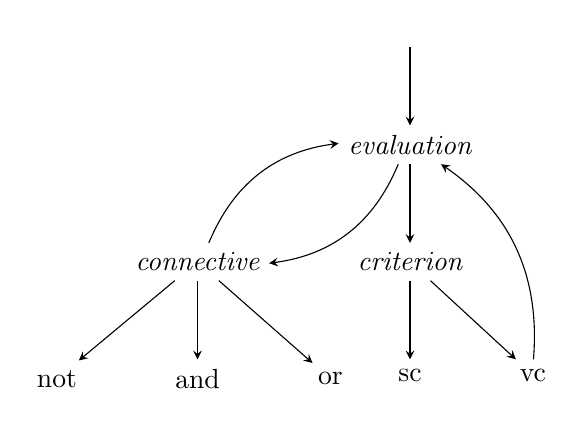
\begin{tikzpicture}[%
            ->,
            >=stealth
        ]
        \node (evaluation) {\itshape evaluation};
        \node[above=of evaluation] (start) {};
        \node[below=of evaluation] (criterion) {\itshape criterion};
        \node[left=of criterion] (connective) {\itshape connective};
        \node[below=of connective] (and) {and};
        \node[right=of and] (or) {or};
        \node[left=of and] (not) {not};
        \node[below=of criterion] (sc) {\glstext{sc}};
        \node[right=of sc] (vc) {\glstext{vc}};

        \path
            (start) edge (evaluation)
            (evaluation) edge (criterion)
            (evaluation) edge[bend left]  (connective)
            (connective) edge[bend left] (evaluation)
            (criterion) edge (sc)
            (criterion) edge (vc)
            (vc) edge[bend right] (evaluation)
            (connective) edge (not)
            (connective) edge (and)
            (connective) edge (or);
    \end{tikzpicture}
\end{figure}
\Glspl{sc} as well as \glspl{vc} evaluate the current state of the simulation or some \gls{av} and determine whether it fulfills a certain condition.
\Glspl{sc} always yield either \iltrue{} or \ilfalse{}.
\Glspl{vc} restrict whether the nested criterion has to be considered during the verification process described in \autoref{sec:testCycle}.
If the condition of the \gls{vc} is \iltrue{} the inner criterion is evaluated and the \gls{vc} returns its result.
Otherwise the \gls{vc} returns \ilunknown{}.
The introduction of \glspl{vc} allows to evaluate different criteria under different circumstances.
Considering a fail criterion like ``While \gls{av} \(A\) drives on lane \(L\) it must not exceed a speed limit of \(S\)'' the speed of \(A\) should only be evaluated as long as \(A\) drives on \(L\) and return either \iltrue{} or \ilfalse{}.
If \(A\) is not on \(L\) \ilunknown{} shall be returned.
The supported types of criteria are based on the formalization of tests and the data \glspl{adas} need as shown in \autoref{tab:reqData}.
The list of supported criteria is in \autoref{table:criteriaTypes}.
Additional criteria can be introduced as explained in \autoref{sec:runtimeVerification}.\par
\begin{table}
    \centering
    \caption{%
        Types of criteria --- This table lists all supported types of test criteria, describes their purpose and lists whether these can be used as \glspl{vc} or \glspl{sc}.
    }
    \medskip
    \begin{tabularx}{\linewidth}{l X c c}
        \toprule
        \bfseries Type & \bfseries Description & \bfseries \glstext{vc} & \bfseries \glstext{sc} \\
        \midrule
        position & Checks whether an \gls{av} is at a certain position or within a certain radius of it & \checkmark{} & \checkmark{} \\
        area & Checks whether an \gls{av} is within a certain area & \checkmark{} & \checkmark{} \\
        lane & Checks whether an \gls{av} drives on a certain lane or off-road & \checkmark{} & \checkmark{} \\
        speed & Checks whether the speed of an \gls{av} is below a given velocity & \checkmark{} & \checkmark{} \\
        damage & Checks whether an \glspl{av} is damaged & \checkmark{} & \checkmark{} \\
        time & Checks whether the simulation is currently within a certain interval of ticks & \checkmark{} & \ding{53} \\
        distance & Checks whether the distance between two \glspl{av} or between an \gls{av} and the center of the lane driving on is smaller than a given distance & \checkmark{} & \checkmark{} \\
        \glstext{ttc} & Checks whether the \gls{ttc} of an \gls{av} and another participant or obstacle is smaller than a given value & \checkmark{} & \ding{53} \\
        light & Checks whether an \gls{av} activated certain lights \eg{} high beam and passing light & \checkmark{} & \checkmark{} \\
        waypoint & Checks whether an \gls{av} has passed a certain waypoint & \checkmark{} & \checkmark{} \\
        \bottomrule
    \end{tabularx}\label{table:criteriaTypes}
\end{table}
\begin{figure}
    \caption{%
        Example criteria definition --- This list shows example definitions for all types of criteria listed in \autoref{table:criteriaTypes}.
        The tag names are built from one of the prefixes ``vc'' or ``sc'' and the type name of the criterion.
        To spare duplication the prefix ``x'' is used here to denote that the criterion can be a \gls{vc} as well as a \gls{sc}.
    }\label{fig:exampleCriteria}
    \medskip
    \lstinputlisting[language=xml]{code/exampleCriteria.dbc.xml}
\end{figure}
{\bfseries Proposed tools:} The whole formalization will be based on \gls{xml} since it has great support in many languages and can be validated based on \glspl{xsd} making sure a test case is specified properly before running it.

\subsection{Test Life Cycle}\label{sec:testCycle}
The test life cycle divides into \textcolor{blue}{input validation}, \textcolor{magenta}{extraction}, \textcolor{cyan}{transformation} and \textcolor{red}{execution} as shown in \autoref{fig:testCycle}.\\
\begin{figure}
    \centering
    \caption{%
        Test life cycle --- Visualizes the four main steps the processing of a test case follows.
        The input validation step is \textcolor{blue}{blue}, the extraction step is \textcolor{magenta}{magenta}, the transformation step is \textcolor{cyan}{cyan} and the execution step is \textcolor{red}{red}.
    }\label{fig:testCycle}
    \medskip
    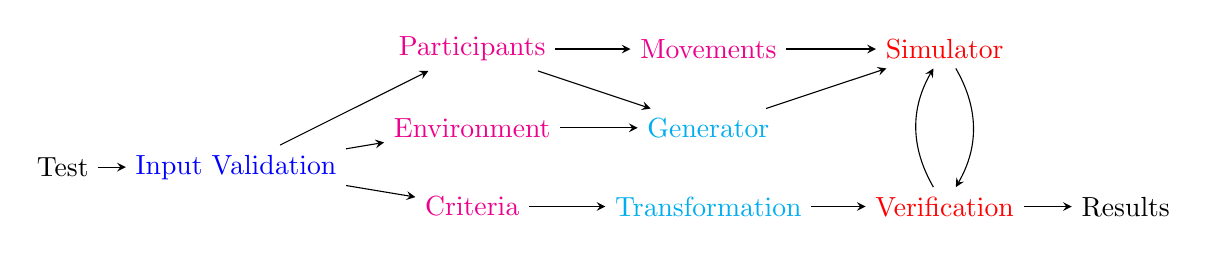
\begin{tikzpicture}[%
            ->,
            >=stealth
        ]
        \node at (-3.2,0) (Tester) {Test};
        \node at (-1,0) (Validation) {\textcolor{blue}{Input Validation}};
        \node at (2,0.5) (Environment) {\textcolor{magenta}{Environment}};
        \node at (2,1.5) (Participants) {\textcolor{magenta}{Participants}};
        \node at (5,1.5) (Movements) {\textcolor{magenta}{Movements}};
        \node at (2,-0.5) (Criteria) {\textcolor{magenta}{Criteria}};
        \node at (5,-0.5) (Transform) {\textcolor{cyan}{Transformation}};
        \node at (5,0.5) (Generation) {\textcolor{cyan}{Generator}};
        \node at (8,1.5) (Simulation) {\textcolor{red}{Simulator}};
        \node at (8,-0.5) (Verification) {\textcolor{red}{Verification}};
        \node at (10.3,-0.5) (Results) {Results};
        \path
            (Tester) edge (Validation)
            (Validation) edge (Environment)
            (Environment) edge (Generation)
            (Generation) edge (Simulation)
            (Validation) edge (Participants)
            (Participants) edge (Movements)
            (Movements) edge (Simulation)
            (Participants) edge (Generation)
            (Validation) edge (Criteria)
            (Criteria) edge (Transform)
            (Transform) edge (Verification)
            (Verification) edge[bend left] (Simulation)
            (Simulation) edge[bend left] (Verification)
            (Verification) edge (Results);
    \end{tikzpicture}
\end{figure}
The input validation checks whether the test case is broken or malformed based on the appropriate \glspl{xsd}.
If the test case is valid the environment, the criteria and the participants are extracted.
The information about lanes and obstacles in the environment is passed to the generator creating representations compatible with the simulator.
The generator also creates a participant for each specified initial state and adds it to the simulation.
The movements of the participants are passed to the simulator that applies these sequentially after the simulation started.
\draft{TODO Mention triggers in the simulation?}
The defined criteria are transformed to a Kleene and Priest logics expression that can be evaluated by the verification process during the simulation.
Then the simulator starts the test and the interaction with the verification process.
This interaction is described more detailed in \autoref{sec:runtimeVerification}.
As soon as the verification process determined whether the test succeeded or failed it stops the simulation and returns the test results.

{\bfseries Proposed tools:} I will use \beamng{}~\cite{beamNG} as simulator since it provides very accurate physics and therefore accurate test results plus it comes with the Python interface BeamNGpy~\cite{beamngpy} that allows to control simulator instances, to create scenarios dynamically and to retrieve sensor data from participants.
Furthermore \beamng{} comes with the ability of pixel perfect annotation which some \glspl{adas} need.
The input validation, the extraction, the generator, the transformation and the verification will be done in Python since the interface of \beamng{} is written in Python too and thus the interaction is easy and the interoperability is high.

\subsection{Runtime Verification}\label{sec:runtimeVerification}
The runtime verification implements the interaction between a simulator and the verification of test criteria deciding whether a test succeeded or failed.
It follows the synchronous simulation strategy to make sure that the point in time where \glspl{ai} have to control \glspl{av} is not influenced by network latency or the current load of the underlying hardware.
\begin{figure}
    \centering
    \caption{%
        Runtime verification --- Depicts the main execution loop of the interaction between a simulator and a verification process (See \autoref{fig:testCycle}).
    }\label{fig:runtimeVerification}
    \medskip
    \smartdiagram[flow diagram:horizontal]{%
        Verify criteria, Request \glspl{ai}, Control, Start Resume, Pause
    }
\end{figure}
The main execution loop realizing synchronous simulation is shown in \autoref{fig:runtimeVerification}.\\
The runtime verification starts with evaluating the preconditions, success and fail criteria and determines the verification result based on the state machine shown in \autoref{fig:verificationDecision}.
\begin{figure}
    \centering
    \caption{%
        Verification state machine --- Shows the state machine for determining the current state of the test case execution based on the evaluation of preconditions, success and fail criteria.
        Underlined nodes are final states and arrows describe the transition from node to node depending on whether a criterion evaluated to \textcolor{green}{true}, \textcolor{red}{false} or \textcolor{blue}{unknown}.
    }\label{fig:verificationDecision}
    \medskip
    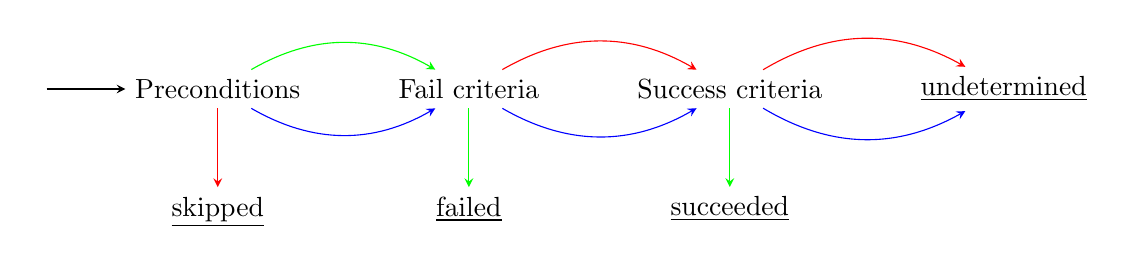
\begin{tikzpicture}[%
        ->,
        >=stealth
    ]
    \node (start) {};
    \node[right=of start] (preconds) {Preconditions};
    \node[below=of preconds] (skipped) {\underline{skipped}};
    \node[right=of preconds] (fail) {Fail criteria};
    \node[below=of fail] (tcFail) {\underline{failed}};
    \node[right=of fail] (success) {Success criteria};
    \node[below=of success] (tcSuccess) {\underline{succeeded}};
    \node[right=of success] (undetermined) {\underline{undetermined}};

    \path (start) edge (preconds);
    \draw[red] (preconds) edge (skipped);
    \draw[green] (preconds) edge[bend left] (fail);
    \draw[blue] (preconds) edge[bend right] (fail);
    \draw[green] (fail) edge (tcFail);
    \draw[red] (fail) edge[bend left] (success);
    \draw[blue] (fail) edge[bend right] (success);
    \draw[green] (success) edge (tcSuccess);
    \draw[red] (success) edge[bend left] (undetermined);
    \draw[blue] (success) edge[bend right] (undetermined);
    \end{tikzpicture}
\end{figure}
If the verification ends in one of the final states \code{SKIPPED}, \code{FAILED}, \code{SUCCEEDED} or \code{TIMEOUT} the simulation stops and returns the final state.
In this case all \glspl{ai} registered at the simulation are told to stop too.
Otherwise the verification yields \code{UNKNOWN} and the runtime verification continues with the main execution loop.
If the runtime verification continues it searches for all \glspl{av} that are according to their movement currently controlled by an \gls{ai} and that have to be requested according to the request frequency and the current time of the simulation (in ticks).
Using the connections \glspl{ai} opened at \drivebuild{} the runtime verification requests them for commands controlling the simulator or an \gls{av} associated with them.
\autoref{fig:aiSimProtocol} depicts the four-way protocol which is used for the communication.
The first message registers an \gls{ai} at a simulation waiting for being requested.
Its response response contains the current state of the simulation which is either \code{RUNNING}, \code{FINISHED}, \code{CANCELED}, \code{TIMEOUT} or \code{UNKNOWN}.
This allows an \gls{ai} to recognize whether the simulation still runs or stopped.
If the simulation still runs the \gls{ai} requests properties of the current state of the associated \gls{av} and its available sensor data needed for the calculations of the \gls{ai}.
%\draft{FIXME List available data?}
The response to these requests contains the appropriate data in a serialized form.
After receiving the data the \gls{ai} starts to calculate control commands for either controlling the simulator (\eg{} interrupt it) or for controlling the associated \gls{av} with values for acceleration, brake intensity and steering angle.
The opportunity to send commands controlling the simulator instead of the \gls{av} allows an \gls{ai} to evaluate additional constraints that extend the specified test criteria and thus eventually force a test to succeed, fail or to be skipped.\\
The control step applies the commands the runtime verification received appropriately to the simulator or the correct \gls{av}.
If the simulator does not get a command to stop it starts the test case execution respectively resumes it if it was paused previously.
The simulator calculates the next tick, pauses the simulation and the runtime verification starts over again.

{\bfseries Proposed tools:} The exchange of messages and data will be based on \protobuf~\cite{protobuf} since it allows to define messages in a programming language neutral way and is able to cross compile classes for serializing messages in many languages including Python.
\begin{figure}
    \centering
    \caption{Communication between a simulation controller and an \glstext{ai} --- Visualizes the messages sent for exchanging data between a simulator and an \glstext{ai}.}\label{fig:aiSimProtocol}
    \medskip
    \includegraphics[page=1]{pictures/aiSimCommunication.pdf}
\end{figure}

\subsection{Cluster Architecture}
The architecture uses a client server model and is depicted in \autoref{fig:systemArch}.
\autoref{fig:distributeNodes} shows the distribution of the system over the cluster.
\begin{figure}
    \centering
    \caption{%
        Cluster architecture --- Visualizes all components of the cluster and the data flow between them.
        The components in the blue area belong to the client side and the components in the green area belong to the cluster.
        The orange area contains cluster components that build the micro service based accessible interface.
        \draft{FIXME Still StatsManager?}
    }\label{fig:systemArch}
    \medskip
    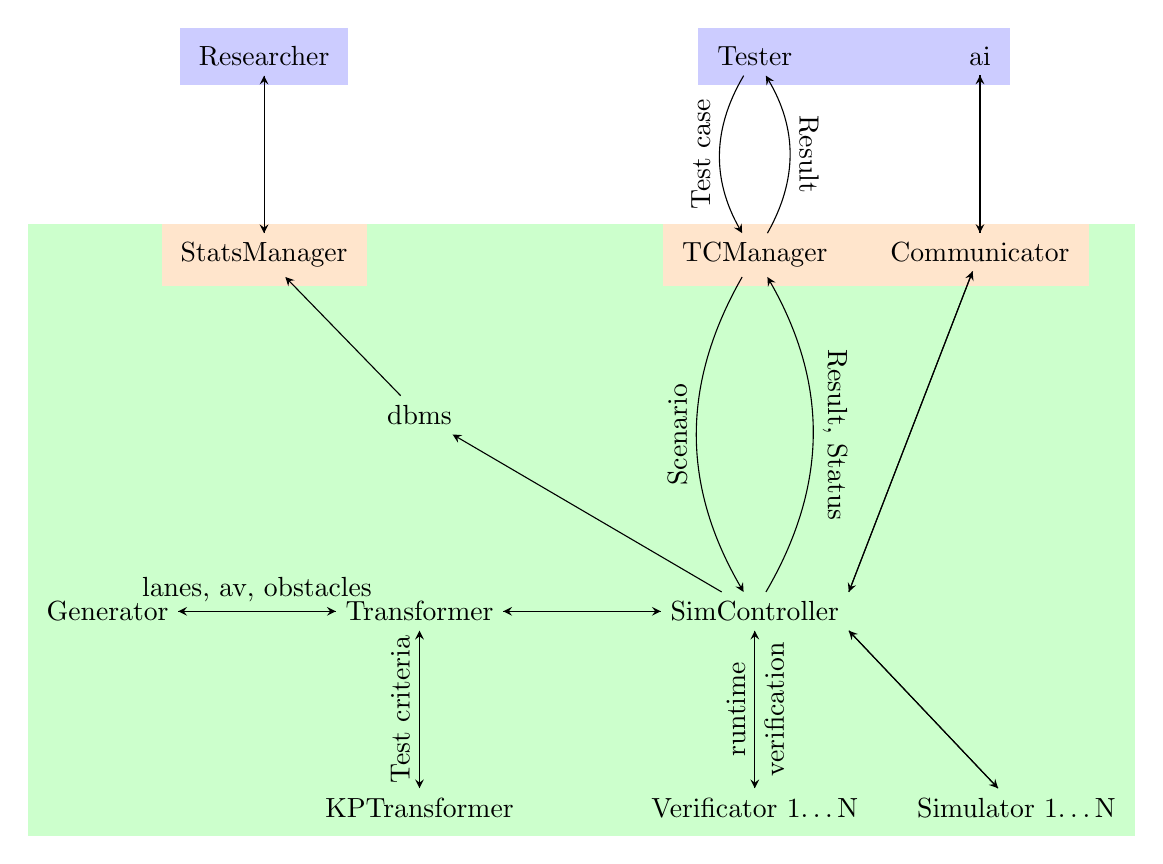
\begin{tikzpicture}[%
        ->,
        >=stealth
    ]
    \tikzset{%
        node distance=2
    }
    \node (tester) {Tester};
    \node[below=of tester] (tcmanager) {TCManager};
    \node[right=of tester] (ai) {\glstext{ai}};
    \node[below=of ai] (communicator) {Communicator};
    \node[below=4 of tcmanager] (simcontroller) {SimController};
    \node[left=of simcontroller] (transformer) {Transformer};
    \node[left=of transformer] (generator) {Generator};
    \node[above=of transformer] (dbms) {\glstext{dbms}};
    \node[left=4 of tcmanager] (stats) {StatsManager};
    \node[above=of stats] (researcher) {Researcher};
    \node[below=of transformer] (kptransformer) {KPTransformer};
    \node[below=of simcontroller] (verificator) {Verificator 1\ldots N};
    \node[right=0.5 of verificator] (simulatorA) {Simulator 1\ldots N};

    \node[zlayer=back,fill=blue!20,fit={(researcher)}] (clientLeft) {};
    \node[zlayer=back,fill=blue!20,fit={(tester)(ai)}] (clientRight) {};
    \node[zlayer=back,fill=green!20,fit={(simulatorA)(communicator)(dbms)(stats)(kptransformer)(tcmanager)(verificator)(generator)}] (server) {};
    \node[zlayer=back,fill=orange!20,fit={(tcmanager)(communicator)}] (microserviceA) {};
    \node[zlayer=back,fill=orange!20,fit={(stats)}] (microserviceB) {};

    \path
        (tester) edge[bend right] node[rotate=90,above]{Test case} (tcmanager)
        (dbms) edge (stats)
        (stats) edge (researcher)
        (researcher) edge (stats)
        (simcontroller) edge (dbms)
        (simcontroller) edge (transformer)
        (transformer) edge (simcontroller)
        (tcmanager) edge[bend right] node[rotate=-90,above]{Result} (tester)
        (transformer) edge node[rotate=90,above]{Test criteria} (kptransformer)
        (kptransformer) edge (transformer)
        (transformer) edge node[above]{lanes, \glspl{av}, obstacles} (generator)
        (generator) edge (transformer)
        (tcmanager) edge[bend right] node[rotate=90,above]{Scenario} (simcontroller)
        (simcontroller) edge[bend right] node[rotate=-90,above]{Result, Status} (tcmanager)
        (simcontroller) edge node[rotate=90,above]{runtime} (verificator)
        (verificator) edge node[rotate=90,below]{verification} (simcontroller)
        (simcontroller.south east) edge (simulatorA)
        (simulatorA) edge (simcontroller.south east)
        (simcontroller.north east) edge (communicator)
        (communicator) edge (simcontroller.north east)
        (communicator) edge (ai)
        (ai) edge (communicator);
    \end{tikzpicture}
\end{figure}
The functionality of the cluster is provided through micro services~\cite{microServices}.
The use of micro services allows hiding and strictly separating functionality plus it allows more granularity than other architectures like \gls{soa}.
The cluster offers multiple services.\\
The TCManager service implements methods for accepting test cases of a tester, checking their validity, passing them to the transformer, triggering the execution of test cases, monitoring the execution, returning test case results to the tester and to store results in a \gls{dbms}.
The Transformer (transformation step in \autoref{fig:testCycle}) accepts validated test cases, extracts information about the environment and the participants, generates representations which are compatible with the simulator, extracts the test criteria and transforms them to an expression that can be evaluated during the simulation.
The SimController manages all simulator instances as well as their verification instances and implements the runtime verification described in \autoref{sec:runtimeVerification}.
It also provides methods for requesting the current status of test executions which the TCManager requires for monitoring.
The Communicator service handles the exchange of messages between a simulation controlled by the SimController and an \gls{ai} controlling an \gls{av} of a scenario and thus uses the protocol visualized in \autoref{fig:aiSimProtocol}.
\draft{FIXME Still StatsManager?}
The StatsManager service grants access to the data stored by the TCManager in the \gls{dbms} enabling researchers to investigate and analyze collected data about test case executions.\par

\begin{figure}
    \centering
    \caption{%
        Distribution over the cluster --- Visualizes how the components shown in \autoref{fig:systemArch} are distributed over multiple nodes.
        The blue node represents a client node, the orange node represents a \gls{vm} providing the micro service layer and the green nodes represent the cluster nodes as well as the \gls{dbms}.
    }\label{fig:distributeNodes}
    \medskip
    \begin{tikzpicture}[%
            ->,
            >=stealth
        ]
        \node (client) {\includegraphics[width=.125\linewidth]{pictures/computer_client.png}};
        \node[right=1.5 of client] (microService) {\includegraphics[width=.125\linewidth]{pictures/virtualMachine_microService.png}};
        \node[right=1.5 of microService] (windows2) {\includegraphics[width=.0625\linewidth]{pictures/virtualMachine_windows.png}};
        \node[above=0.5 of windows2] (windows1) {\includegraphics[width=.0625\linewidth]{pictures/virtualMachine_windows.png}};
        \node[below=0.25 of windows2] (dots) {\vdots};
        \node[below=0.25 of dots] (windows3) {\includegraphics[width=.0625\linewidth]{pictures/virtualMachine_windows.png}};
        \node[right=1.5 of windows2] (dbms) {\includegraphics[width=.0625\linewidth]{pictures/dbms.png}};

        \node[below=0.2 of windows3] (windowsTitle) {Cluster};
        \node[right=1.3 of windowsTitle] (dbmsTitle) {\glstext{dbms}};
        \node[left=1.2 of windowsTitle] (microServiceTitle) {MicroServices};
        \node[left=1.8 of microServiceTitle] (clientTitle) {Client};

        \draw
            (client) edge (microService)
            (microService) edge (client)
            (microService) edge (windows1)
            (windows1) edge (microService)
            (microService) edge (windows2)
            (windows2) edge (microService)
            (microService) edge (windows3)
            (windows3) edge (microService)
            (dbms) edge (windows1)
            (windows1) edge (dbms)
            (dbms) edge (windows2)
            (windows2) edge (dbms)
            (dbms) edge (windows3)
            (windows3) edge (dbms)
            (microService) edge[bend left=70] (dbms) % FIXME These two edges needed?
            (dbms) edge[bend right=70] (microService);
    \end{tikzpicture}
\end{figure}

{\bfseries Proposed tools:} I will use \postgresql{} since many languages provide good support, it is well known and thus bullet proven.
The micro services will be based on Flask~\cite{flask} since it is written in Python providing high compatibility with other components and it allows to use \gls{html} templates.\draft{FIXME Templates relevant?}

    %!TEX root = ../proposal.tex
\section{Planned Evaluation}
The evaluation divides into a quantitative and a qualitative part.
The dataset will be collected during the seminar ``Search-based Software Engineering for Testing Autonomous Cars'' at the university of Passau which takes place in the summer term 2019.

%\draft{%
%    The qualitative part investigates whether the proposed formalization for test cases is a capable of describing all proposed \glspl{adas}.\\
%    FIXME Can the result be ``surprising'' in any way?\\
%    Investigate which \glspl{adas} can be described?
%}
%
%\draft{Investigate accuracy of load prediction somehow?}
%
%\draft{%
%    How to test runtime overhead with external \glspl{ai}?
%    How does efficiency of protocol change with an increasing amount of data?\\
%    Is it interesting?
%    Could it be surprising?\\
%    Main factor: network latency\\
%    Well\ldots Having an \gls{ai} externally is slower than having it on the same machine\ldots\\
%}
%
%\draft{%
%    Check runtime behavior of verification with an increasing number of test criteria?
%    This may be too complicated to check (Many diverse criteria, depth of criteria,\ldots).\\
%    First, run simulation with runtime verification.
%    Secondly, run it the same amount of ticks but without runtime verification.
%    A comparison should yield the runtime overhead of the verification.
%}
%
%\draft{Check calculation time for ticks with an increasing number of participants?}
%
%\draft{%
%    Is the remote/synch approach feasible for multiple \glspl{ai}?
%    Basically\ldots
%    Yes.
%    It is explicitly designed for that.
%    I don't see any reason why this could go wrong (at least none that could be evaluated within the thesis).
%}
%
%\draft{%
%    Is the formalization able to handle automatic test generation?
%    Is there any reason for the formalization to care about whether a test case was generated or written by hand?
%    Everything can be generated automatically but the \glspl{ai} itself and their access points.
%    What is ``type of generation''?
%}
%
%\draft{The simulator needs especially good GPUs \(\Rightarrow\) \Gls{ram} is not interesting}

\subsection{Quantitative Analysis of Runtime Verification}
The quantitative analysis evaluates the runtime complexity of the test criteria verification based on the complexity of the lanes and the complexity of test criteria definitions.\\
The complexity of the lane network is defined by the number of waypoints \(N_W\) and the average tolerances \(T_W\).
The higher \(N_W\) and the lower \(T_W\) the more complex is the lane network.\\
The complexity of the test criteria definition is defined by the number of test criteria \(N_C\) and the average depth \(D_C\) where \(N_C\) is the number of \glspl{sc} plus the number of \glspl{vc}.
The higher \(N_C\) and the higher \(D_C\) the more complex is a test criteria definition.\\
The use of \drivebuild{} during the seminar allows to collect much data about test cases and their execution.
Each executed test case is stored in the \gls{dbms} along with their results, statistics about them and the execution times of every call to the test criteria verification.
For the evaluation I will create tuples \((N_W, T_W, N_C, D_C, T)\) for every execution time \(T\).
Based on these I will create four graphs grouping the tuples by \(N_W, T_W, N_C\) or \(D_C\) and averaging over \(T\).
All graphs yield a runtime complexity.\\
In the end, the runtime complexities determine the maximum complexity of test criteria definitions that is feasible and which of \(N_W, T_W, N_C\) and \(D_C\) is the most crucial.
%\draft{(NOTE This is especially interesting for load prediction.)}\\
%\draft{%
%    FIXME What about absolute times?
%    If absolute times are really small the runtime complexity is not as interesting anymore.
%}\\
%\draft{%
%    FIXME Due to lazy evaluation resulting from \glspl{vc}: Do complexity of test criteria definitions and runtime complexity correlate?
%    The runtime complexity may be very dependant on the actual test case.
%}

\subsection{Qualitative Study of Comprehensiveness}
The qualitative study investigates the comprehensiveness of \drivebuild{} in terms of the capabilities of the formalization and the application areas for which \drivebuild{} can be used.
I will ask participants of the seminar (about 11 people) which kinds of test cases they realize, how they use \drivebuild{} for automation, benchmarks and training \glspl{ai} and which problems they had to face or were not able to solve.
When one of the participants encounters a problem I will investigate whether the current system is able to solve it.
If this is not the case I will explore how \drivebuild{} would have to be extended to solve the problem and decide whether I add it.
I will document all of these steps.\\
In the end, this documentation shows the capabilities of \drivebuild{}.
I will be able to show problems of the original system, whether these problems could be solved and how they where solved if added.

    %!TEX root = ../proposal.tex
\section{Schedule}
% The schedule should sum up to 6 months including the time to write the document
% This period is more or less 26/27 weeks.

% Mention the Starting date and the Expected Completion date

% Please check the "booktabs" latex package manual at http://ftp.fernuni-hagen.de/ftp-dir/pub/mirrors/www.ctan.org/macros/latex/contrib/booktabs/booktabs.pdf

The thesis is limited to a maximum time period of 6 months.
Starting at the 13th of May this results in 26 weeks ending on 10th of November.
Since \drivebuild{} is used during the seminar the schedule has to consider the progress of the seminar and requires to result in a working implementation until half of the semester.
The schedule in \autoref{table:schedule} divides into three milestones.
The first milestone contains the collection of requirements and the actual implementation of \drivebuild{}.
In the second milestone I will collect data about the executed tests, conduct my qualitative study and evaluate my work.
In the third milestone I will write the actual thesis.

\begin{table}[h!tp]
\centering
\caption{%
    Thesis Schedule --- Contains all main tasks of my work, how long they presumably take and how these are grouped into milestones.
}
\medskip
\begin{tabularx}{\linewidth}{c X}
\toprule
\bfseries Weeks   & \bfseries Task\\
\midrule
1                 & Specify formalization schemes and \gls{ai} communication protocol\\
1                 & Implement Generator, KPTransformer and Transformer\\
2                 & Implement SimController with runtime verification\\
3                 & Implement Communicator and TCManager\\
Milestone M1      & ``Ready to go''\\
\midrule
4                 & Implement collection of data and StatsManager\\
5 --- 12          & Conduct and document qualitative study, collect data for quantitative analysis and provide support and bugfixes\\
End of semester\\
13 --- 16         & Analyze qualitative study\\
17                & Conduct quantitative analysis\\
Milestone M2      & ``Final countdown''\\
\midrule
18 --- 24         & Refine and finalize thesis\\
25 --- 26         & Contingency time of 2 weeks\\
Milestone M3      & ``Final destiny''\\
\bottomrule
\end{tabularx}\label{table:schedule}
\end{table}

After the 26th week there are 2 days left until the available time is fully used.
These are planned to print the thesis and hand it in.

    %!TEX root = ../proposal.tex
\section{Success criteria}
The system to develop shall satisfy all Must-Have requirements to be considered as successful.
\begin{description}
    \item[Requirement R1] The system shall be able to convert a given formalized test scenario into a \beamng{} scenario.
        The simulation shall contain roads, traffic participants and obstacles and shall simulate the movement specified in the test case.
    \item[Requirement R2] The system shall be able to simulate multiple generated \beamng{} scenarios simultaneously.
    \item[Requirement R3] The system shall be able to continuously evaluate test criteria during simulation time.
    \item[Requirement R4] The system shall collect executed test cases and their execution results.
    \item[Requirement R5] The system shall measure the execution time of test criteria verifications. \draft{FIXME Really?}
    \item[Requirement R6] The system shall provide a service granting access to the collected data. \draft{FIXME StatsManager?}
\end{description}

The system should implement May-Have criteria to further increase the capabilities provided to users of the system.
\begin{description}
    \item[Requirement M1] The system should provide predefined test suites for training \glspl{ai}.
\end{description}

This work will neither focus nor implement the following aspects.
\begin{description}
    \item[Requirement N1] The system will not support test cases that require real time capabilities.
    \item[Requirement N2] The system will not support running simulations on various Linux distributions or MacOS.
    \item[Requirement N3] There will not be the opportunity to simulate participants with a custom shape and physics that are not provided by the simulator.
    \item[Requirement N4] The system will not be able to create log files for replaying and debugging simulations \eg{} ROSBAG files.
\end{description}


    \pagebreak

    \section{References}
    \begingroup
    \renewcommand{\section}[2]{}%
    \printbibliography[category=cited]
    \endgroup

%    \section{Not cited}
%    \begingroup
%    \renewcommand{\section}[2]{}%
%    \printbibliography[notcategory=cited]
%    \endgroup
\end{document}
